We now investigate whether word orders as found in natural language reflect optimization for the memory--surprisal trade-off more generally.
To this end, we compare the memory--surprisal trade-offs of 52 actual languages to those of counterfactual baseline languages, which differ from the actual languages only in their word order rules. This method of comparison against counterfactual baseline languages was introduced by \citet{gildea-optimizing-2007,gildea-grammars-2010} has been applied to study optimization-based models of word order universals by \citet{futrell-large-scale-2015}, \citet{gildea-human-2015}, and \citet{hahn2020optimization}.

Here, we describe how we measure the memory--surprisal trade-off in corpora, and how we generate counterfactual baseline languages. In Section~\ref{sec:main-experiment-results}, we compare the trade-off in real corpora against the trade-off in the counterfactual baselines. For the majority of languages, we find that the real languages have more favorable memory--surprisal trade-offs than the baselines, in line with our Main Hypothesis.

\subsection{Measuring the memory--surprisal trade-off in corpora}

The key to evaluating the memory-surprisal tradeoff from corpus data is the set of quantities $I_t$ (defined in Section~\ref{sec:infoloc}), the  mutual information between words at distance $t$ conditional on the intervening words. 
All that is required is to estimate the quantities $I_t$; then these can be plugged in to Theorem~\ref{prop:suboptimal} to give a lower bound on the memory--surprisal trade-off. 

The quantities $I_t$ can be estimated as the difference between the average surprisal of Markov models that have access to the last $t-1$ or $t$ words.
That is, if we have a $t$th-order Markov model with average surprisal
\begin{equation*}
    S_t = H[w_t | w_0, \dots, w_{t-1}]
\end{equation*}
and a $(t-1)$th-order Markov model with average surprisal
\begin{equation*}
    S_{t-1} = H[w_t | w_1, \dots, w_{t-1}],
\end{equation*}
then we can calculate $I_t$ straightforwardly in the following way:
\begin{align}
    \nonumber
    I_t &= I[w_t : w_0 | w_1, \dots, w_{t-1}] \\
    \nonumber
    &= S_{t-1} - S_t.
\end{align}
Therefore, to evaluate $I_t$, all we need is a way of fitting Markov models of order $t$ and $t-1$ and computing their average surprisals.

To fit Markov models to the data, we use neural language models. In particular, we use Recurrent Neural Networks with Long Short-Term Memory architectures \citep{hochreiter-long-1997}. 
Neural network models are the basis of the state-of-the art in statistical modeling of language and in predicting the surprisal effect on reading times~\citep{frank-insensitivity-2011,goodkind-predictive-2018}.
See Supplementary Materials Section X for details on how these models were fit to data, and see Supplementary Materials Sections Y and Z for control studies using other methods of estimating $I_t$ (based on $n$-gram models and PCFG chart parsers). The results of these control studies are in agreement with the neural network results presented in this section.

In order to evaluate the average surprisal values $S_t$, we computed the empirical word-by-word surprisal values under the $t$th-order Markov model for held-out data, different from the data that was used to train the model. By evaluating on held-out data, we avoid underestimating the value of $S_t$ due to overfitting.

\subsection{Data}
We draw on corpora annotated with syntactic structures.
The Universal Dependencies project has compiled such annotated corpora for several dozen languages~\citep{nivre-universal-2017}.
These are annotated in the format of Dependency Grammar.

\paragraph{Dependency Grammar}
In dependency corpora, sentences are annotated with \emph{dependency trees} (Figure~\ref{fig:dependency}).
These are directed trees describing the grammatical relations among words. For example, the arcs labeled ``obj'' represent that the noun in question is the \emph{direct object} if the verb, rather than e.g. the subject or an indirect object.
A dependency arc is drawn from a \emph{head} (e.g. TODO in Figure TODO) to a \emph{dependent} (e.g. TODO).
Dependency trees can be defined in terms of many different syntactic theories \citep{corbett1993heads}.
Although there are some differences in how different formalisms would draw trees for certain sentences, there is broad enough agreement about dependency trees that it has been possible to develop large-scale dependency-annotated corpora of text from dozens of languages \citep{nivre2017universal}.

\begin{figure}
\centering
\begin{dependency}[theme = simple]
   \begin{deptext}[column sep=1em]
	   I \&	   wrote \& risāla \& li \& sadīq  \\
   \end{deptext}
	%   \deproot{3}{ROOT}
   \depedge{1}{2}{obj}
	%   \depedge[edge start x offset=-6pt]{2}{5}{ATT}
   \depedge{1}{4}{obl}
   \depedge{4}{3}{case}
   %\depedge[arc angle=50]{7}{6}{ATT}
\end{dependency}
	\caption{TODO Dependencies example}\label{fig:dependency}
\end{figure}

\paragraph{Selection of Languages}
We considered all languages for which there are Universal Dependencies 2.4 treebanks with a total of at least 500 sentences of training data.
We excluded data from historical languages.\footnote{Historical languages excluded: Ancient Greek, Classical Chinese, Coptic, Gothic, Latin, Old Church Slavonic, Old French.}
%While running this experiment, data from additional languages became available that also had enough data, through the Universal Dependencies 2.4 release. 
This resulted in 54 languages.

\paragraph{Processing of Corpora}
For each of these languages, we pooled all available corpora in one dataset.
We excluded corpora that primarily contain code-switched text\footnote{Hindi English corpus}, or text created by non-native speakers.\footnote{ESL for English, CFL for Chinese.}
Most Universal Dependencies corpora have a predefined split into \emph{training}, \emph{held-out} (also known as \emph{development}), and \emph{test} partitions.
%While larger corpora have all three partitions, smaller corpora often have only some of these partitions.
In most cases, we used the predefined data split, separately pooling data from the different partitions. 
For some languages with little data, there is no predefined training partition, or the training partition is smaller than the other partitions.
In these cases, we redefined the split to obtain more training data.
For these languages, we pooled all the available partitions, used 100 randomly selected sentences as held-out data, and used the remainder as training data.\footnote{This affects Amharic, Armenian, Breton, Buryat, Cantonese, Faroese, Kazakh, Kurmanji, Naija, Thai, and Uyghur.}
We did not make use of the \textit{test} partitions here.
We provide the sizes of the resulting datasets in Table~\ref{tab:corpora}.

\subsection{Defining baselines}

We construct counterfactual ordering grammars that define consistent ordering rules similar to those found in actual languages.
For instance, these grammars will specify which dependents precede or follow their heads (e.g., whether objects follow or precede verbs, whether adjectives follow or precede nouns), and the relative order of different dependents on the same side of the head (e.g., whether noun phrases have order adjective-numeral-noun or numeral-adjective-noun). Our formalism of ordering grammars adapts the method of \citet{gildea-optimizing-2007,gildea-grammars-2010,gildea-human-2015} to the setting of dependency corpora, following \citet{futrell-large-scale-2015} and \citet{hahn2020optimization}, among others.


\begin{figure}
\centering
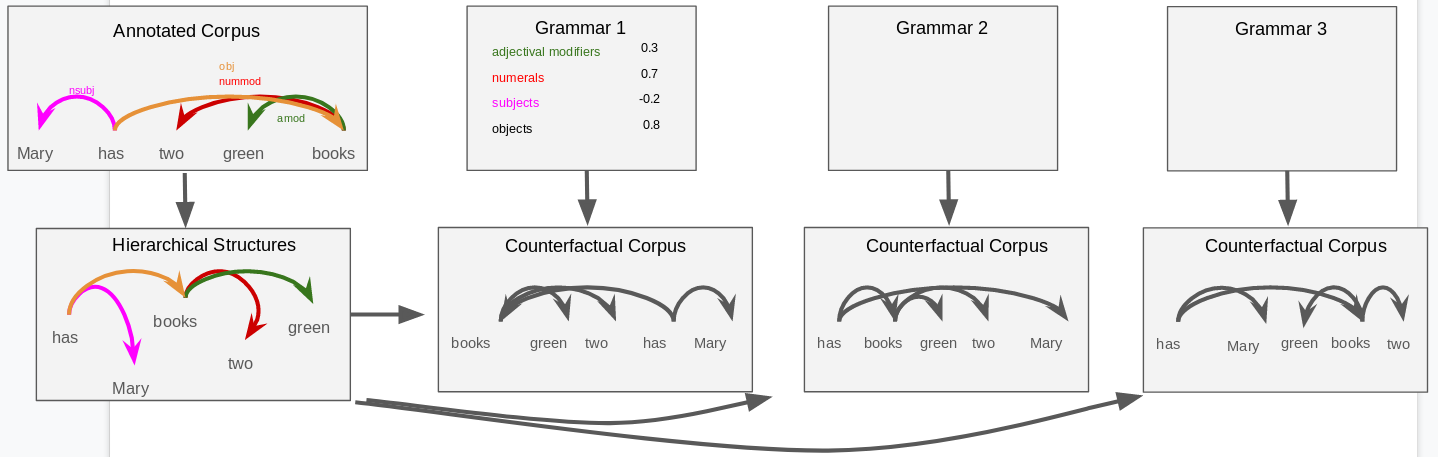
\includegraphics[width=\textwidth]{figures-gdrive/counterfactual-languages.png}
	\caption{\note{Can say more here to explain how it works} Estimating chance by constructing counterfactual grammars and languages.\jd{this figure is again blurry for me. also looks like there's sth in the background on the left?}}\label{fig:grammars}
\end{figure}


Universal Dependencies 2.4 defines 37 universal syntactic relations that are used to label dependency arcs across all corpora.
These relations encode cross-linguistically meaningful relations such as subjects, objects, and adjectival modifiers.
We define ordering grammars by assigning a parameter $a_\tau \in [-1,1]$ to every one of these 37 universal syntactic relations.
Relations sometimes have language-specific subtypes; we do not distinguish these subtypes.

Following Gildea and colleagues, this parameter defines how dependents are ordered relative to their head:
Given a head and a set of dependents, we order each dependents by the parameter $a_\tau$ assigned to the syntactic relation linking it to the head.
Dependents with negative weights are placed to the left of the head; dependents with positive weights are placed to the right.

Ordering grammars describe languages that have consistent word order:
For instance, the subject is consistently ordered before or after the verb, depending on whether the parameter for the verb-subject dependency is positive or negative.

We construct baseline grammars by randomly sampling the parameters $a_\tau$.
Such baseline grammars define languages that have consistent word order, but do not exhibit systematic preferences for specific word order patterns such as short dependencies.


In actual languages, the ordering of words is largely determined by the syntactic relations (CITE).
However, certain kinds of rules cannot be modeled by our word order grammars, such as rules sensitive to the category of the dependent (e.g., differences between nominal and pronominal objects).
Word order freedom also is not modeled.
In this sense, ordering grammars represent approximations to the kinds of ordering rules found in natural language \citep{gildea-optimizing-2007, gildea-grammars-2010, gildea-human-2015}.
See Section (Discussion) for further discussion.


We first constructed at least 10 baseline grammars for each of the 54 real languages.
We then continued to construct baseline grammars until a precision-based stopping criterion was reached (CITE). This criterion was designed to ensure that enough grammars were sampled to reliably compare the tradeoff curves of real and baseline grammars, without biasing results towards or against our hypothesis (see SI).

\subsection{Results}

\begin{figure}
	\begin{center}
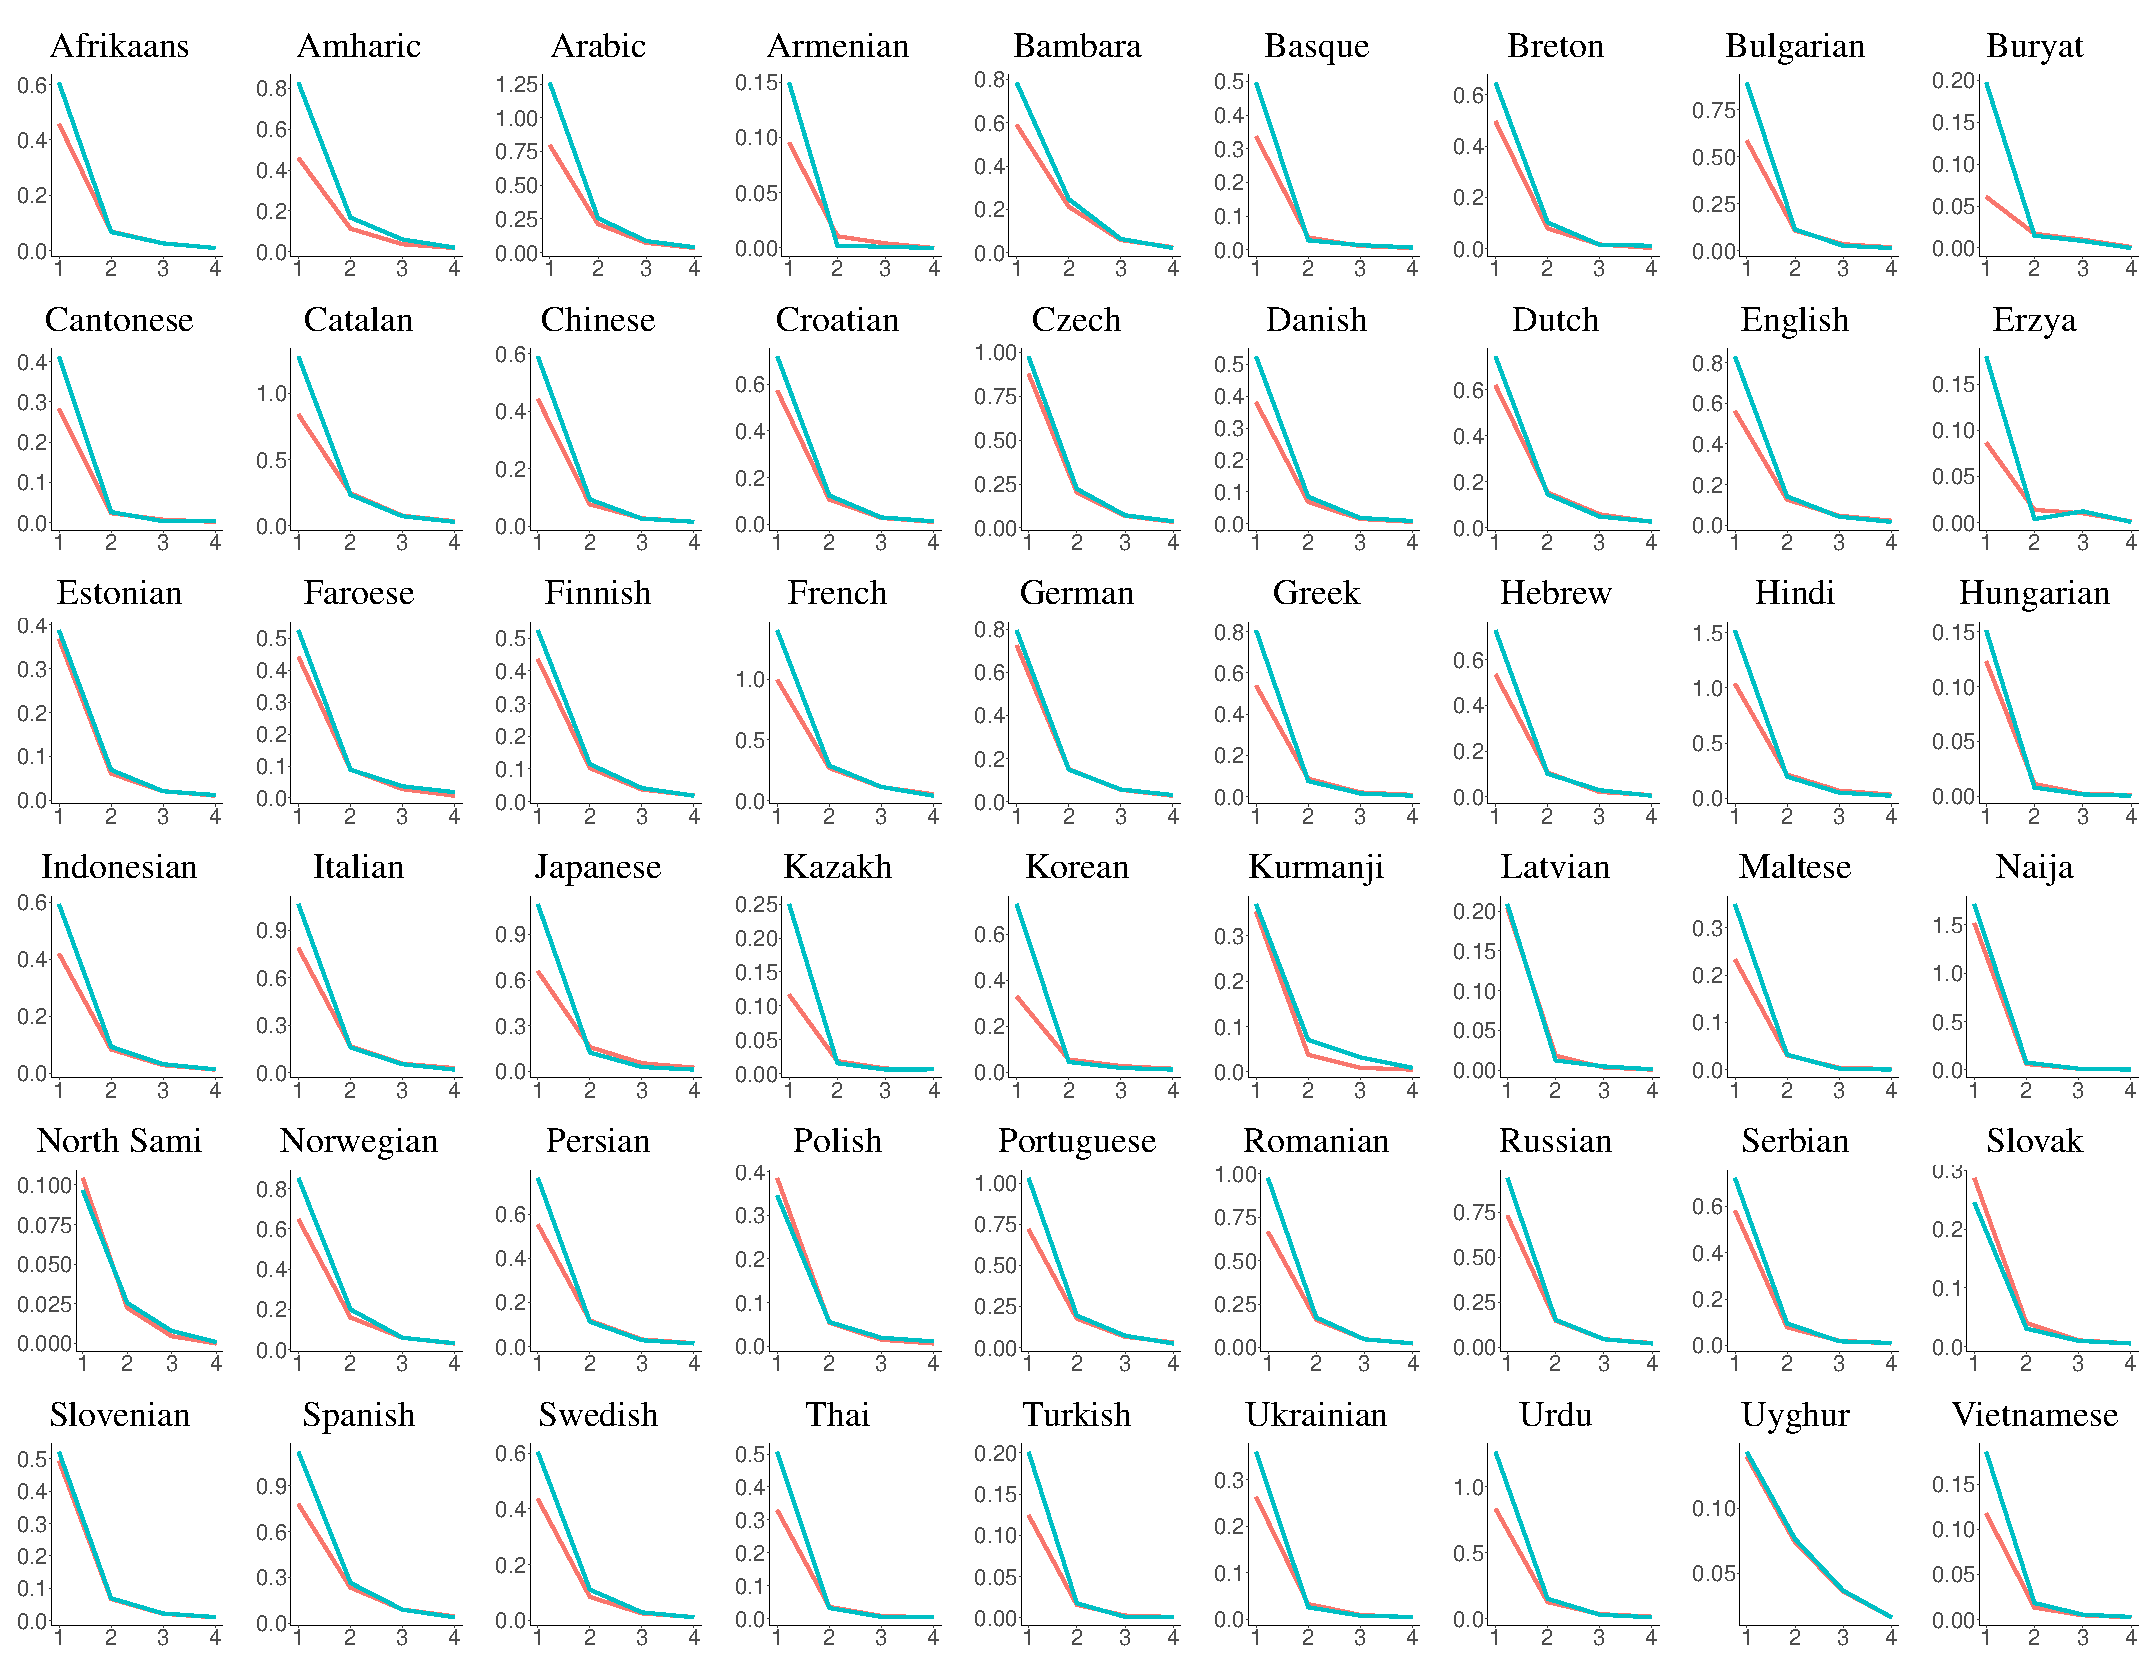
\includegraphics[width=\textwidth]{it-table.pdf}
\end{center}
	\caption{$I_t$ (y-axis) as a function of $t$ (x-axis), for real (blue) and counterfactual (red) orders. We plot the median over all runs of the neural network estimator, and over all random grammars.}\label{fig:it}
\end{figure}



\begin{figure}
	\begin{center}
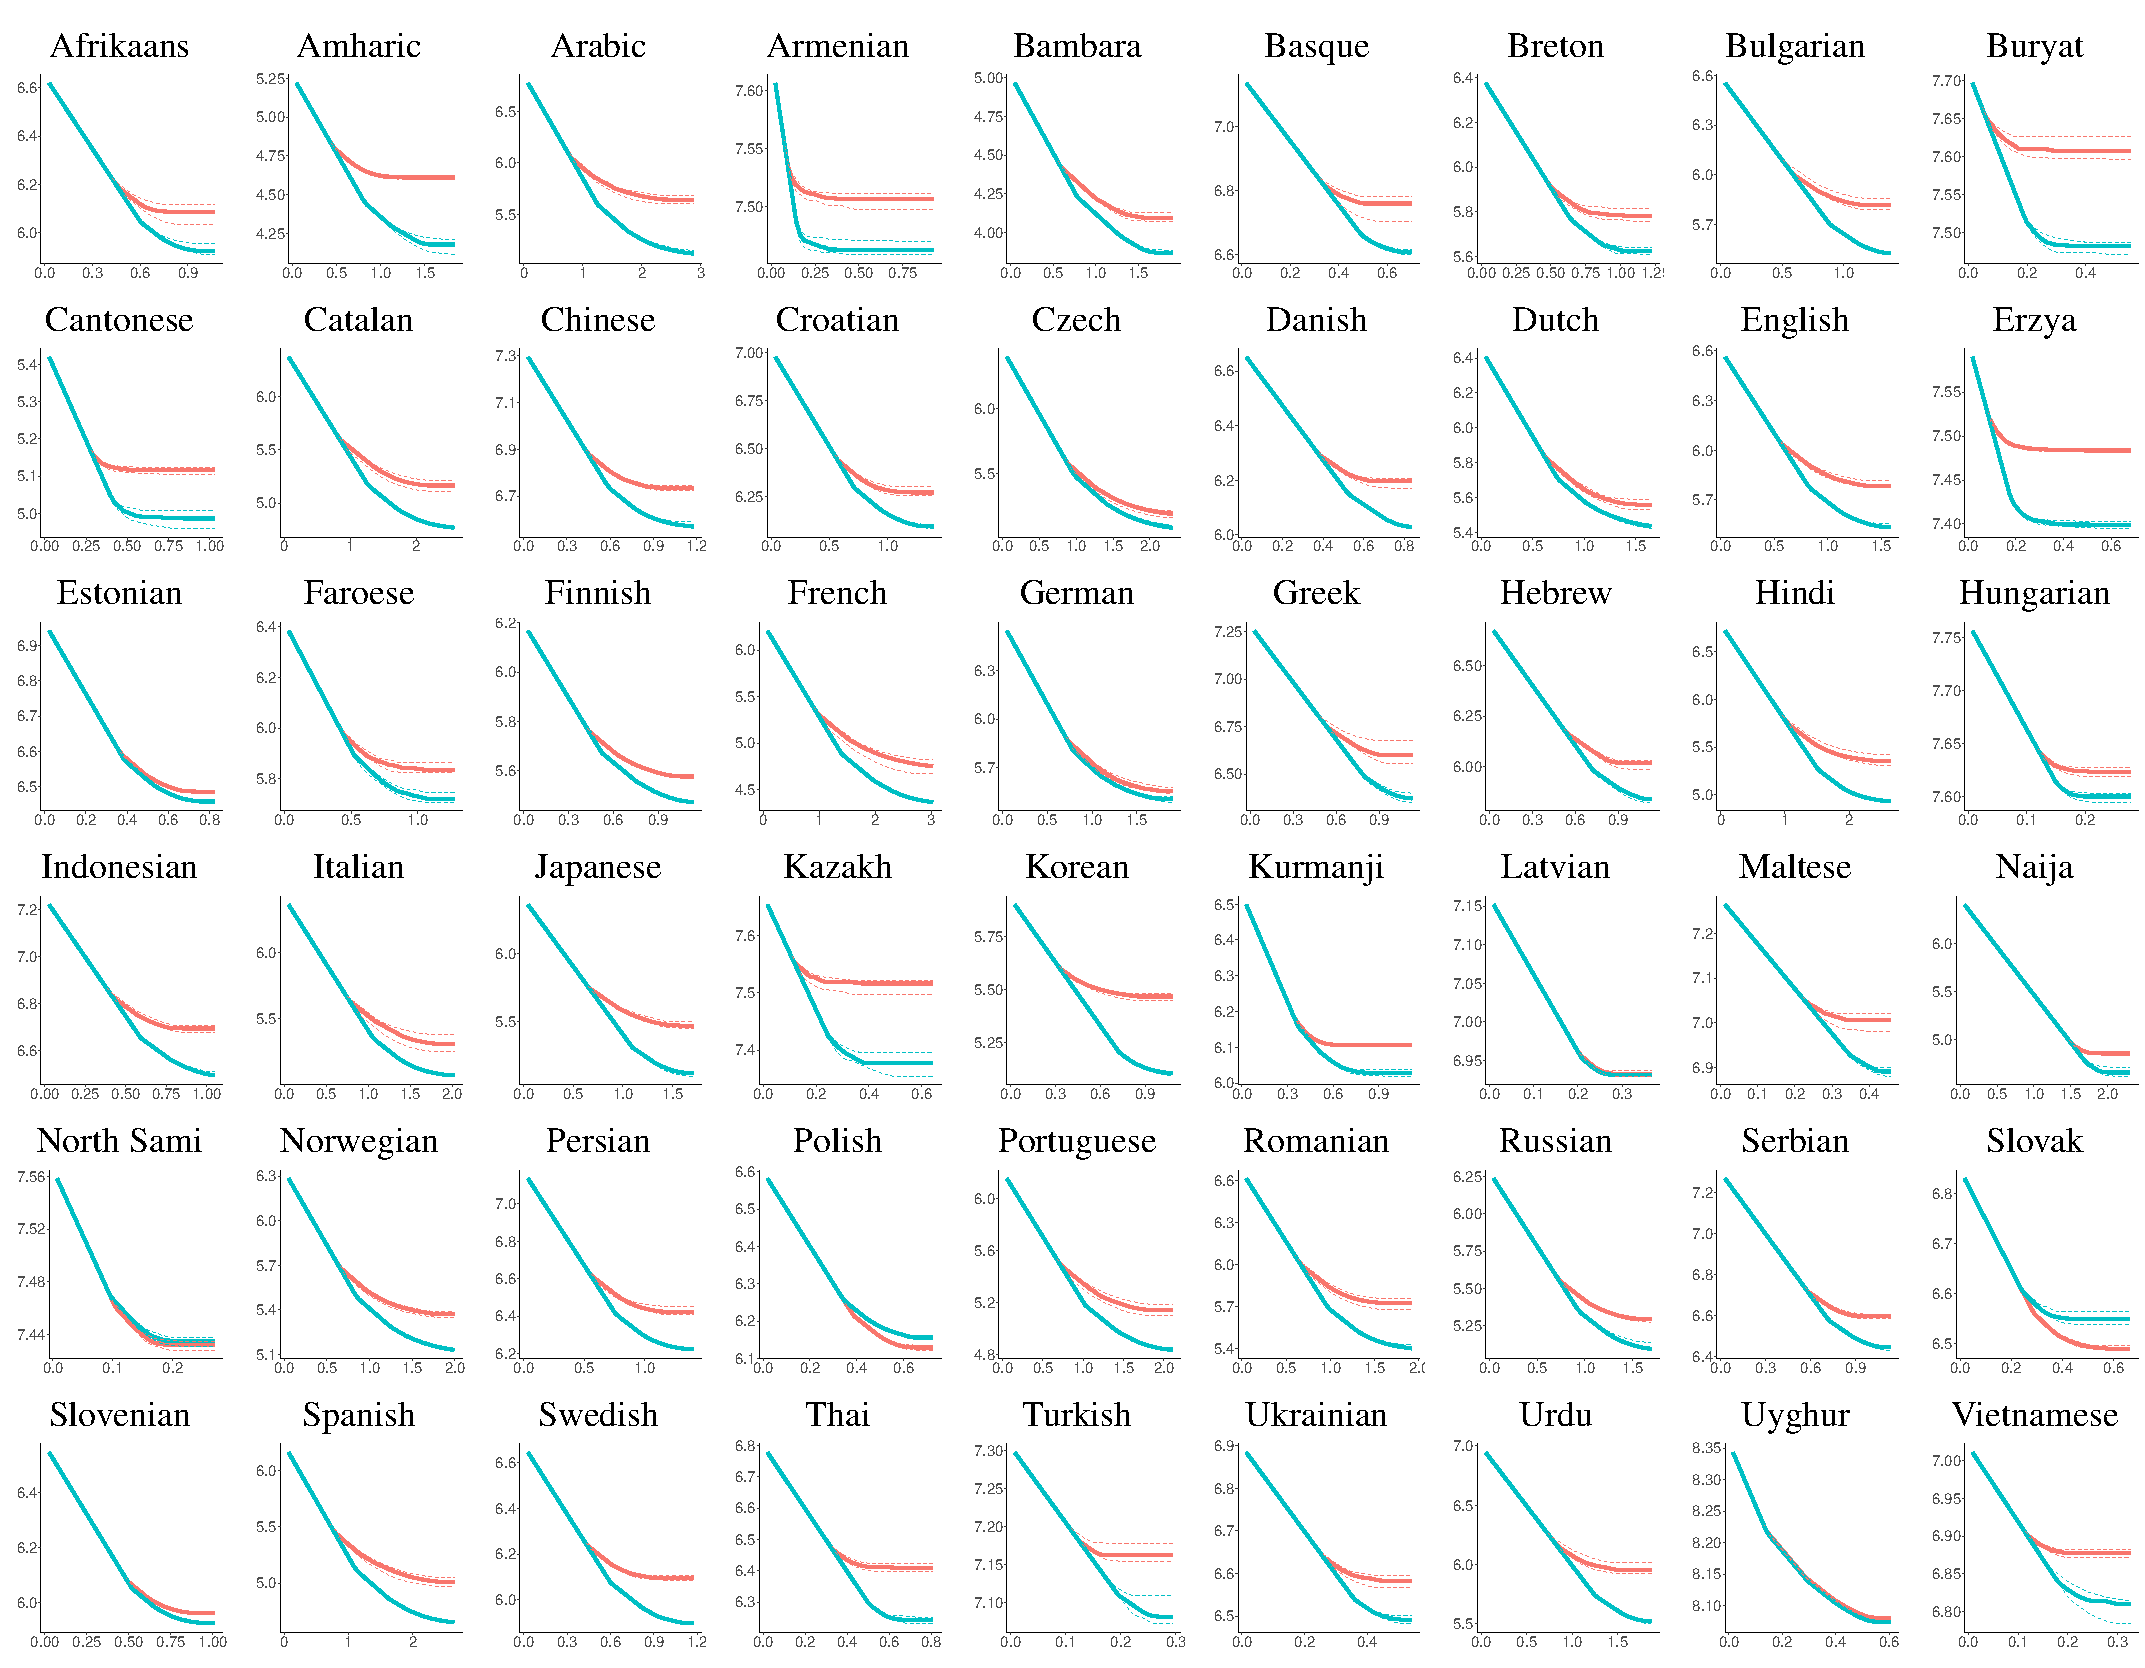
\includegraphics[width=\textwidth]{results-table.pdf}
\end{center}
	\caption{Median surprisal (y-axis) at given memory level (x-axis), for real orders (blue) and random baseline grammars (red). We provide 95\% confidence bands. These are computed over different runs of the estimation algorithm for the real orders, and over different runs \emph{and} different grammars for the baseline grammars.}\label{fig:median-table}
\end{figure}


\begin{figure}
	\begin{center}
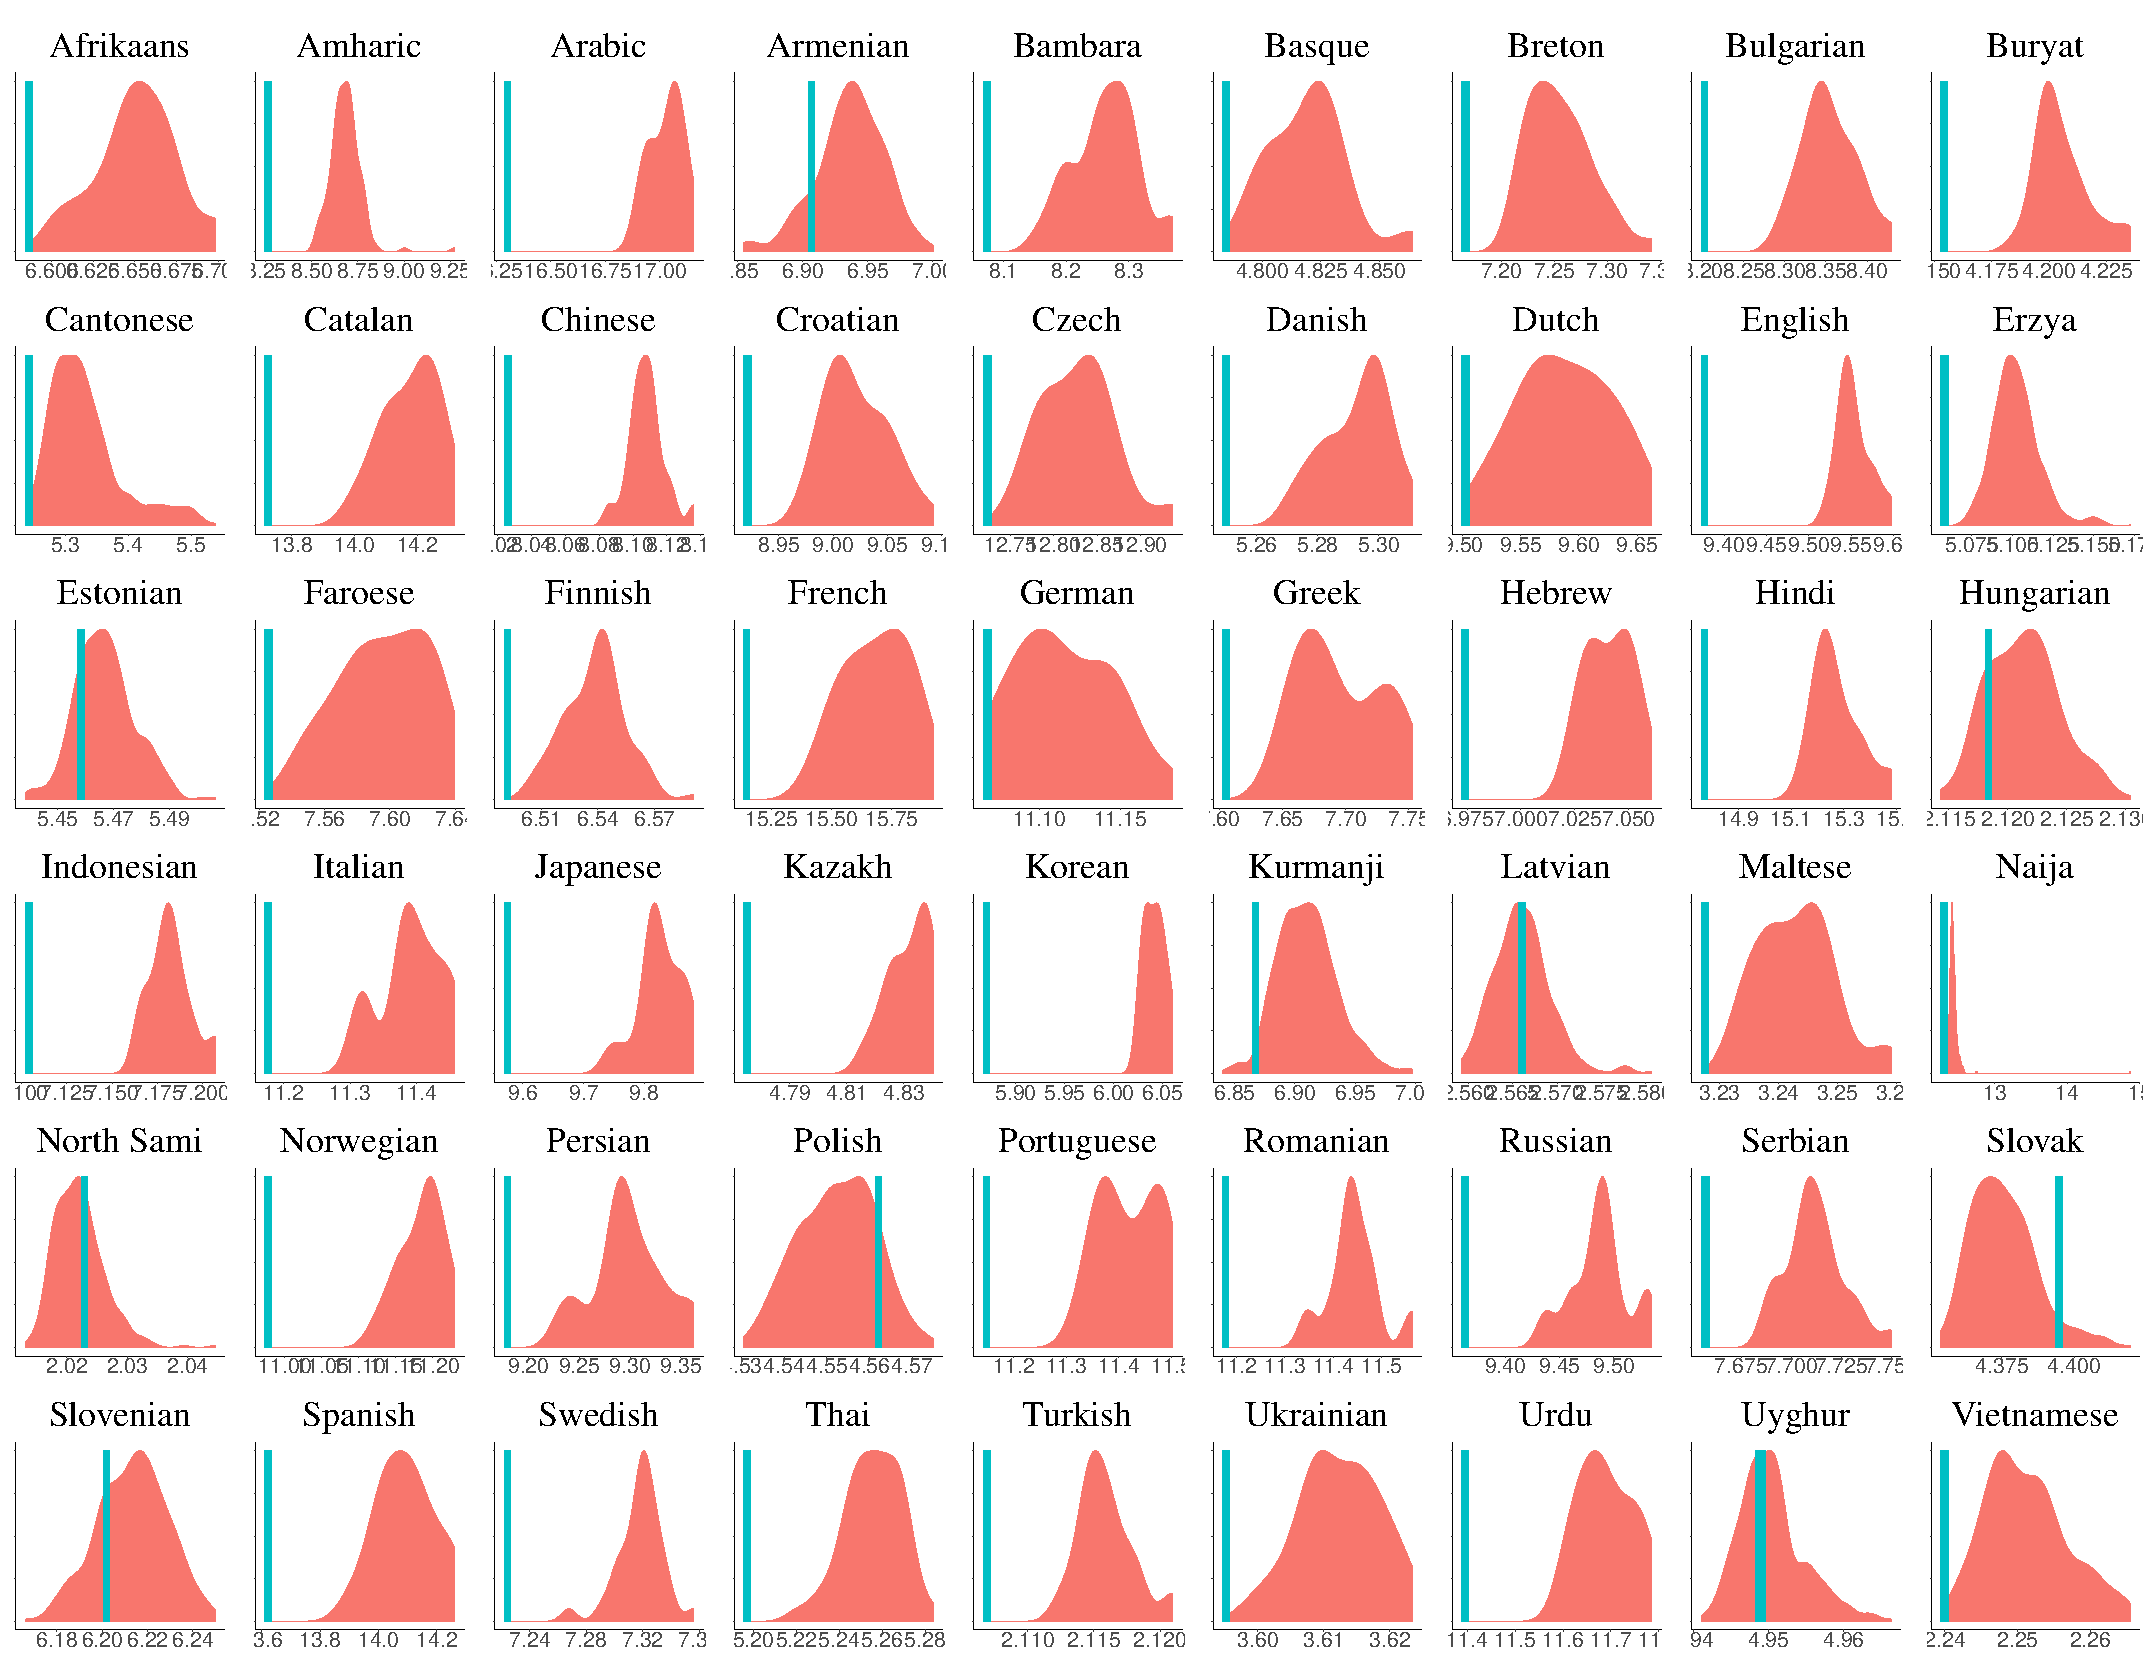
\includegraphics[width=\textwidth]{auc-table.pdf}
\end{center}
	\caption{AUC Histograms}\label{fig:auc}
\end{figure}






In Figure~\ref{fig:it}, we show the estimated values of $I_t$ for real orders (blue) and the median of $I_t$ across different baseline grammars (red).
In most languages, $I_1$ is distinctly larger for the actual orderings (blue) compared to the baseline orderings (red). This means that real orderings tend to concentrate more predictive information at the immediately preceding word than baseline grammars.

In Figure~\ref{fig:median-table}, we show the resulting bounds on the memory-surprisal tradeoff curves, showing median surprisals at given levels of memory, for real and baseline languages.
We compute surprisal at 40 evenly spaced points of memory (selected individually for each language), over real orders and baseline grammars.
We then compute the median surprisal over all runs for the real language, and over all baselines grammars.
For each point, we compute a confidence interval for the median surprisal, using the binomial PDF. \mhahn{some standard stats reference}
This is an \emph{exact} confidence interval, without parametric assumptions or asymptotic approximations.

Numerically, the real language provides better tradeoffs than the median of the baselines across languages, with four exceptions (Latvian, North Sami, Polish, Slovak).


In order to quantify the degree of optimality of real orders, we further computed the area under the memory-surprisal tradeoff curve (AUC) for real and baseline orderings.
Area under the curve (AUC) is a general quantity evaluating the efficiency of a tradeoff curve (CITE).
A \emph{smaller} area indicates a \emph{more efficient} tradeoff.
In Figure~\ref{fig:auc}, we plot the AUC for the real orderings, together with the distribution of AUCs for baseline grammars.
We quantify the degree of optimality by the fraction of baseline grammars for which the AUC is higher than for the real orders:
The real ordering is highly efficient if it results in a lower AUC than almost all baseline grammars.
Numerically, the AUC is smaller in the real orderings than in at least 50\% of baseline grammars in all but three languages (Polish, Slovak, North Sami).
We evaluated significance using a two-sided binomial test.
In these three languages, the AUC is higher in the real orderings than in significantly less than 50\% ($p < 0.01$ in each language).
In all other languages except for Latvian, the fraction of more efficient baseline grammars was significantly less than 50\%, at $p=0.01$ using Hochberg's step-up procedure (CITE).
In 42 of the 54 languages, the fraction of more efficient baseline grammars out of the samples taken was 0\%.



\subsection{Discussion}

We have found that 50 out of 54 languages provide better memory-surprisal tradeoffs than random baselines with consistent but counterfactual word order rules.

Four languages provide exceptions; these are Latvian (Baltic), North Sami (Uralic), Polish and Slovak (both Slavic).
All four languages have strong word order freedom (CITE).
Freedom of word order plausibly makes sentences less predictable, as the same syntactic structure can receive different surface realizations.
We thus hypothesized that freedom of word order impacts the memory-surprisal tradeoff, and that languages with more strongly fixed word order should display more optimal memory-surprisal tradeoffs.

To test this hypothesis, we examined the correlation between word order freedom and the surprisal difference between real and baseline orderings.
To quantify word order freedom, we used a corpus-based estimate, the \emph{branching direction entropy}~\citep{futrell-quantifying-2015}.
This is the entropy of the ordering (head-first or dependent-first) of dependencies conditioned on the dependency label and the part-of-speech label of head and dependent.
These two quantities are plotted in Figure~\ref{fig:hist-real}.
We found that branching direction entropy was strongly correlated with the surprisal difference between real and baseline orderings (Spearman correlations -0.58, $p = 7.414e-6$).

We will address this in Experiment 3.


\begin{figure}
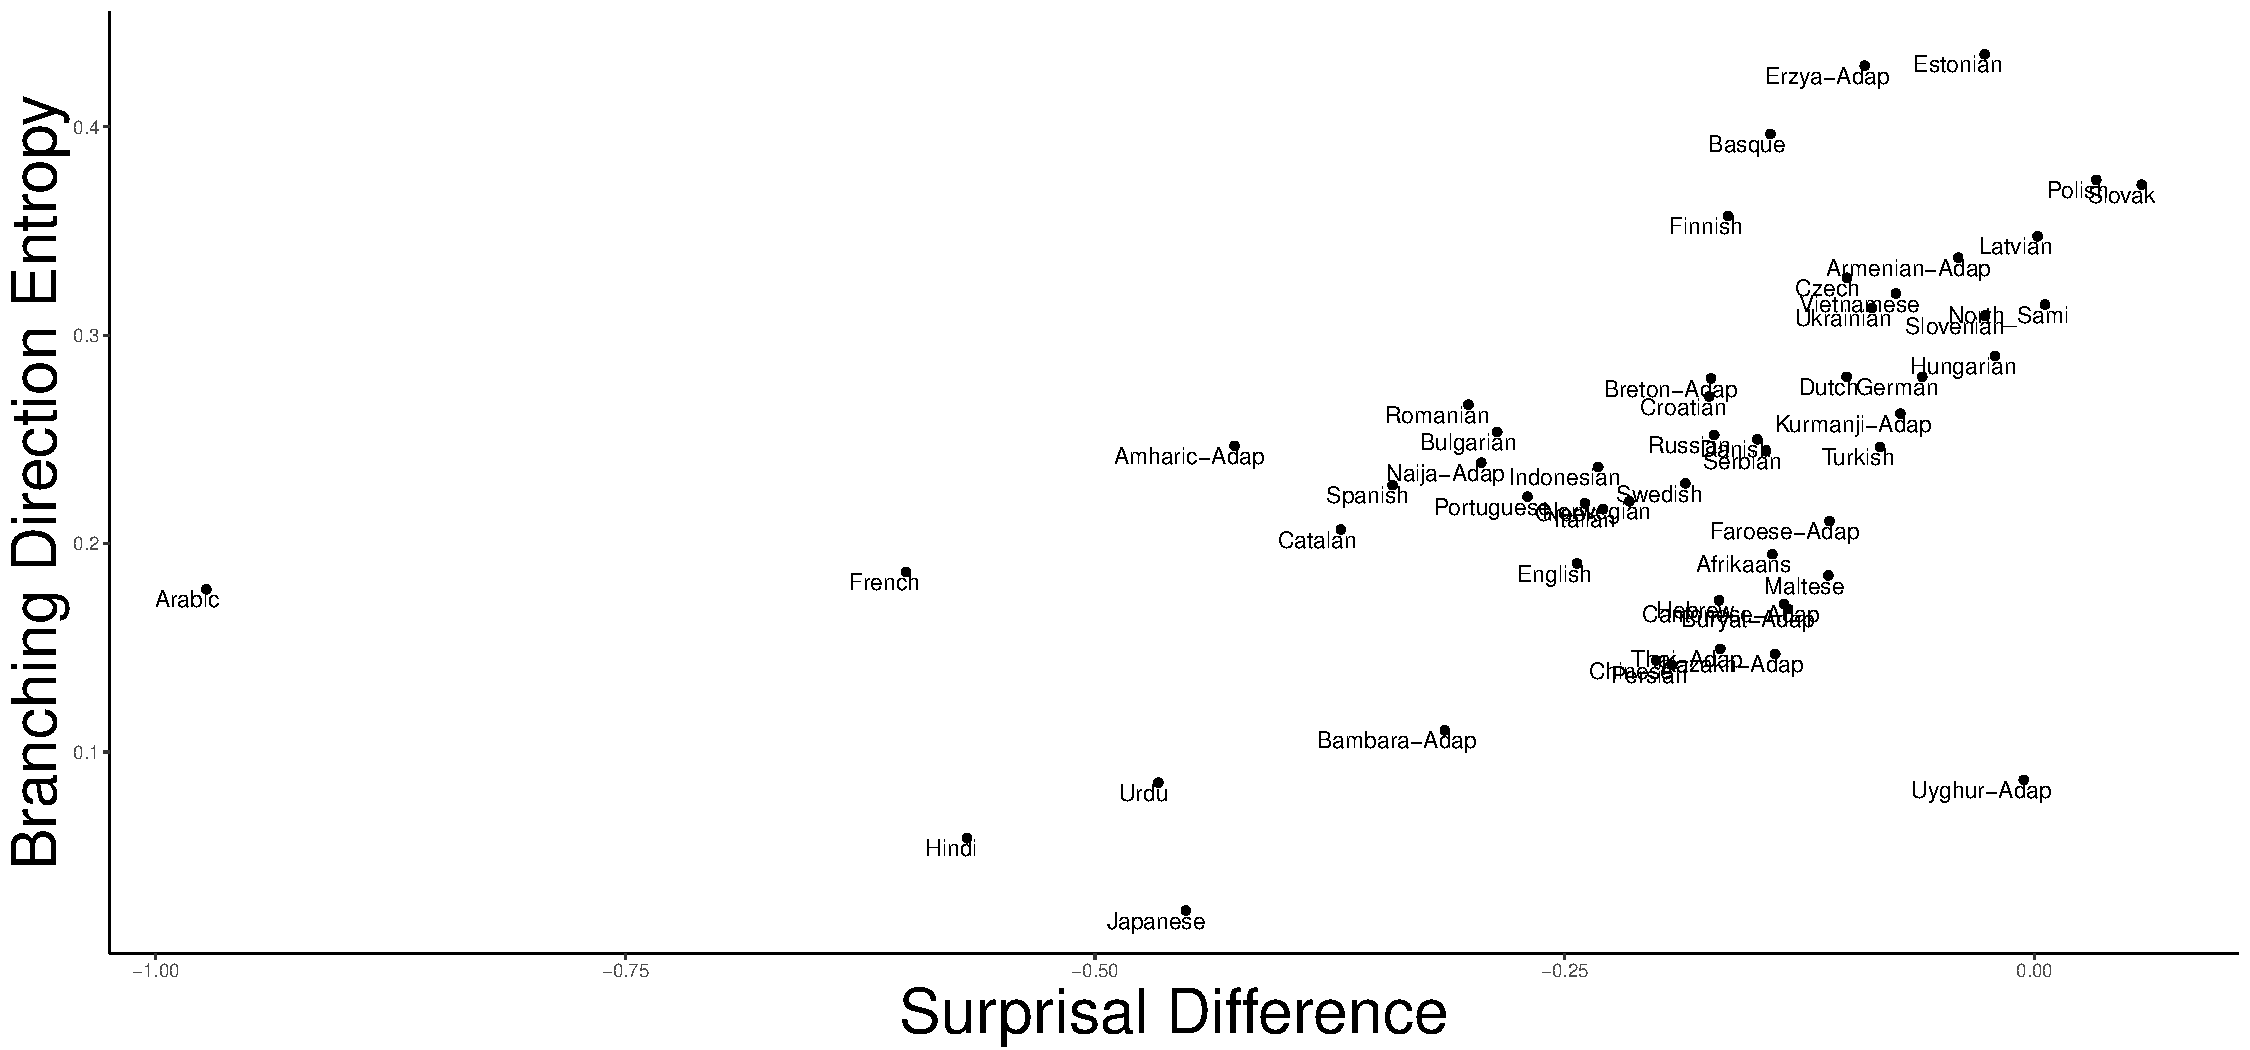
\includegraphics[width=0.95\textwidth]{figures/surprisal-branching-entropy-REAL.pdf}
	\caption{Surprisal Difference vs Branching Direction Entropy.}\label{fig:hist-real}
\end{figure}


\mhahn{One thing that has to be discussed: the absolute values differ between languages}



A possible concern with this experiment that the optimization observed in Experiment 2 might be an artifact of the grammar formalism:
Baseline grammars cannot exactly represented all word order rules found in real languages, and this restriction in representational capacity might potentially impact the optimality of resulting memory-surprisal tradeoffs.
We will address this in Experiment 3 by repeating the experiment comparing baseline grammars to grammars that represent the word order of the real languages as faithfully as is possible with the grammar formalism.


